\def\year{2017}\relax
\documentclass{article}
\usepackage{aaai17}
\usepackage{times}
\usepackage{helvet}
\usepackage{courier}
\frenchspacing
\setlength{\pdfpagewidth}{8.5in}
\setlength{\pdfpageheight}{11in}

\usepackage{comment}
\usepackage{subfigure}
\usepackage{enumitem}
\usepackage[ruled,vlined,linesnumbered]{algorithm2e}
\usepackage{algorithmic}

\usepackage{bm}%used for bm
\usepackage{graphics}
\usepackage{graphicx}
\usepackage{amsmath} %used for maths symbols
\usepackage{amssymb}%used for empty set symbol
\usepackage{url}
\usepackage{xcolor}% or package color

\usepackage{makecell}


\usepackage{multirow}% for table

\newtheorem{rmk}{Definition}% definition

%used for quotes
\usepackage{epigraph}
\setlength\epigraphwidth{\columnwidth}
\setlength\epigraphrule{0pt}

\usepackage{array}
\newcolumntype{L}[1]{>{\raggedright\let\newline\\\arraybackslash\hspace{0pt}}m{#1}}
\newcolumntype{C}[1]{>{\centering\let\newline\\\arraybackslash\hspace{0pt}}m{#1}}
\newcolumntype{R}[1]{>{\raggedleft\let\newline\\\arraybackslash\hspace{0pt}}m{#1}}

\setcounter{secnumdepth}{2}  
 \begin{document}
% The file aaai.sty is the style file for AAAI Press 
% proceedings, working notes, and technical reports.
%
\title{Knowledge Base Enhanced Continous Learning for High Accuracy Event Detection}
\maketitle


%主动感知的
%\title{Is That Enough to Use the Recent Data to Detect Events?}
%\title{Revealing the Important Factors on the High Accuracy Event Detection}

%基于历史的 adoptable continous learning 连续学习for high accuracy event detection
%长轴:military方面的,三个切片,每个切片top10的词都进行展示。起始是维基的导入,连续学习产生了一个长轴。
%关注于重要事件的积累:1,变化很大,2,相当长的稳定性。长轴上的例子,第三个切片需要第一个切片的知识。第三个切片自身产生的很准确。
%两个例子:(1)之前学习的结果对事件检测有帮助(类似于张学良的case);(2)可以扩展词表时新性很好,很准确;

%点明factor是什么——能准确描述历史知识的model,该model的表述能力起码能够model概念和概念之间的联系;model应该有一个实时自学习功能,即在历史知识的基础上,能在不断到来的新数据流上更新自己的知识。(“支持”恐怖组织,“打击”恐怖组织)打击恐怖组织的topic中,通常是美国和英国、法国;但是俄罗斯突然出现在该topic的列表中,说明俄罗斯参与打击恐怖组织应该被判别为一个新的事件。需要一个精确描述历史数据中概念之间联系的例子——(找到一个立场发生变化的例子,如果能在叙利亚问题上找到很好,如果不能考虑别的例子)。

\begin{abstract}

Many web applications need the real time event detection technique. But the accuracy of existing methods are still far from meeting the application requirements. 
%should be met, 这个词应该被强化,vital
We reaveal that the two important factors should be met, (1) having a good mechanism to organize the history data, and (2) having the capability of self-updating, to accumlate the knowledge about what is happening.
%NSDetector的特性应该被
According to this guideline, we propose \textsc{NSDetector}, a high accuracy event detection method that trains normal states better by using knowledge base, which can be treated as the accumulation of history data. 
In \textsc{NSDetector}, 1) a new data structure \textit{normal states} is proposed to restore what happened; 2) \textit{normal states} can be initialized by knowledge base and further updated by upcoming text streams via our proposed probabilistic model NS-Prior-LDA; 3) events can be detected by normal states with high accuracy.
Experiments on the benchmark \textit{Edinburgh twitter corpus (30 million tweets)} validate the effectiveness of our proposed \textsc{NSDetector}.
\textsc{NSDetector} promotes the accuracy rate by 9\% without  sacrificing the recall rate.
%在不牺牲召回率的情况下,将准确率相比于state-of-art提升了9%。


\begin{comment}
Event detection is an important task to understand what already happened and what is currently happening in the rapid evolving text stream. 
% what happened不需要了
% 诸多互联网的应用都迫切需要实时准确的事件检测技术。
% 由于需要实时监测最新发生的事件,人们通常实时分析最新的数据流来检测可能发生的事件,但很遗憾这种技术的准确率远远不能支撑应用的要求。

%举例之后,1这个例子说明需要哪些新技术支持——需要对历史知识有准确的描述,充分体现概念与概念之间的联系;并且能够利用新数据来更新相应的知识,以解决知识库的更新滞后于新数据的问题 2 列举related works,这些技术无法解决这个问题
%我们的工作。

%在Related Works 之前说明我们这是一个amazing的工作,同时将precision和recall都进行了提升,而一般的工作很难兼顾这一点。
But existing methods cannot achieve high precision and high recall simultaneously. 
The reason lies in that they only use the recent data and lack the accumulation of history knowledge. 
We further find out that the ideal event detection method should have two properties: \textit{organizing history data well} and \textit{self-updating}.
According to this guideline, we propose \textsc{NSDetector}, a high accuracy event detection method that trains normal states better by using knowledge base, which can be treated as the accumulation of history data. 
In \textsc{NSDetector}, 1) a new data structure \textit{normal states} is proposed to restore what happened; 2) \textit{normal states} can be initialized by knowledge base and further updated by upcoming text streams via our proposed probabilistic model NS-Prior-LDA; 3) events can be detected by normal states with high accuracy.
Experiments on the benchmark \textit{Edinburgh twitter corpus (30 million tweets)} validate the effectiveness of our proposed \textsc{NSDetector}.
%\textsc{NSDetector} imitates this process automatically in the event detection task, and further verify that the key to improve the accuracy of event detection lies in training the normal states well. 
\end{comment}
\end{abstract}

%\textsc{NSDetector} imitates this process automatically in the event detection task, and further verify that the key to improve the accuracy of event detection lies in training the normal states well. 

\section{Introduction}
Many web applications\cite{ge2015bring}\cite{hughes2009twitter}\cite{sakaki2010earthquake} need the real time event detection technique. 
But the accuracy of existing methods are still far from meeting the application requirements. 
The main stream of existing methods focus on monitoring the changes of the recent data\cite{Allan:2000wu}\cite{Petrovic:2010uj}\cite{Wurzer:2015wq}, and some others use the history data by word frequencies\cite{Li2013JointEE}\cite{Nguyen2015EventDA} and dictionary\cite{Twevent2012}. 
A typical example the existing methods cannot handle well is that ``Russia's anti-ISIS operation in Syria". The word Russia, ISIS, and Syria are trivial, while Russia's anti ISIS is nontrivial because US and other Europe countries but not Russia are the countries that anti ISIS  before September 2015. 
%这个例子应该

To handle this challenge, the important factors on the high accuracy event detection are needed: (1) having a good mechanism to organize the history data, and being aware of what happened; (2) having the capability of self-updating, to accumlate the knowledge about what is happening.

The properties of the ideal event detection method also coincide with the news value theory\cite{galtung1965structure}\cite{caple2013delving}, which emphasizes the \textit{news unexpectedness} -- ``the unpredictable or the rare is more newsworthy than the routine"\cite{bell1991language}, and ``routine events are difficult to assimilate to the news, which favours the novel, the atypical and the unusual"\cite{montgomery2007discourse}.
Following this guideline, if the journalist knew the normal states, aka, the ``routine things" of everyday better, he/she would tend to choose more unexpected news to report. 
We suppose that the ideal event detection system performs like a journalist who can find news from cyberspace with the knowledge of the normal states. 
%Taking another example in our study for example, the tweet ``UN declares famine in Somalia (7/20/2011)"\footnote{\url{https://en.wikipedia.org/wiki/2011_East_Africa_drought}} is related to a \textit{public security} event as the famine has the potential of relating to a war.
%Being aware of the history knowledge, such as \textit{Vietnamese Famine of 1945}\footnote{\url{https://en.wikipedia.org/wiki/Vietnamese_Famine_of_1945}}, \textit{Dutch famine of 1944-45}\footnote{\url{https://en.wikipedia.org/wiki/Dutch_famine_of_1944-45}} caused by World War II, it's possible to detect it accurately. 

It's very close for the ideal event detection method, which holds the previous mentioned two properties (\textit{organizing history data well} and \textit{self-updating}). To implement the ideal event detection method, we propose \textsc{NSDetector}, a high accuracy event detection method that trains normal states better by using knowledge base, which can be treated as the accumulation of happened things. 
In \textsc{NSDetector}, 1) a new data structure \textit{normal states} is proposed to restore what happened; 2) \textit{normal states} can be initialized by knowledge base and further updated by upcoming text streams via our proposed probabilistic model NS-Prior-LDA; 3) events can be detected by normal states with high accuracy.

But the existing computation on the RDF graph is often time consuming. To overcome this obtacle, we propose the new data structure \textit{normal states}, which not only utilize the structure adequately but also maintain the information about what happened and what's happening more efficiently than RDF.  

\begin{figure}[h]
    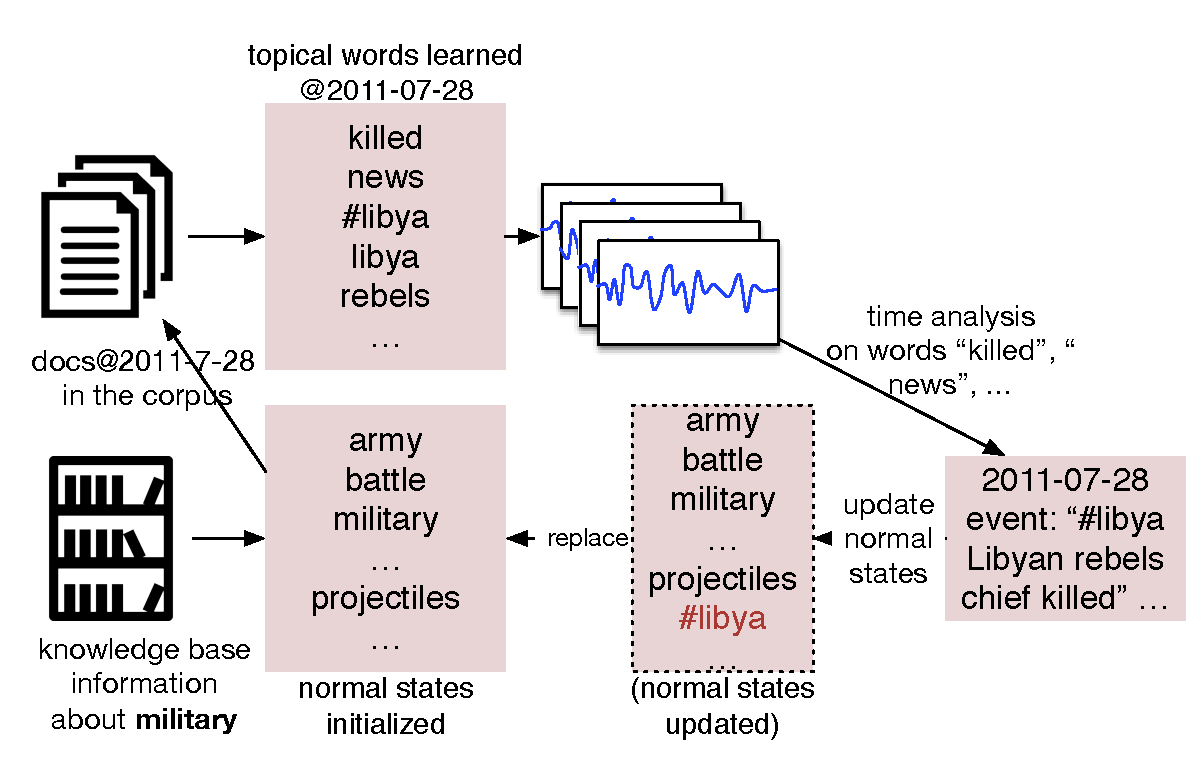
\includegraphics[width=1.0\columnwidth]{img/NSDetectorExample.pdf}
    \caption{\textsc{NSDetector}'s process flow, taking \textit{public security} related events in cyberspace as an example. \textsc{NSDetector} initializes the normal states about military from knowledge base, learns the topical words further within the time windows on the target corpus, detects events, and updates the normal states incrementally by the detected events.}
    \label{fig:modelDesc}
\end{figure}


The contribution of this paper is mainly in three aspects.
(1) We reveal that there are two important factors for high accuracy event detection-- a comprehensive model that can organize history data well, and updating the model well.
(2) We propose the probability model \textsc{NSDetector}. 
The model can combine the history data and the recent data, further determine the arrival new document whether it represents a new event. 
More than that, \textsc{NSDetector} has the capability to update the knowledge of what happend.
(3) The experiment on the Edinburgh twitter corpus which contains 30 million tweets show that \textsc{NSDetector} promotes the accuracy rate by 9\% without sacrificing the recall rate.


\section{Related Works}
The first category of methods, including UMass\cite{Allan:2000wu} and BBTM\cite{yan2015probabilistic}, use \textit{the data within the recent time windows} to help to decide whether the incoming article is related to a new event. 
This kind methods can be implemented by clustering of articles\cite{Allan:2000wu}\cite{Petrovic:2010uj}\cite{Wurzer:2015wq}, word frequencies\cite{Mathioudakis:2010fc}\cite{Weng:2011wz}, or topic modeling\cite{Diao:2012wj}\cite{Yan:2015wm} in the recent time windows. 
Taking the clustering of articles as an example, they model the occurred events as clusters, and link the incoming article with an already existed event cluster or assign it as the new detected event.
The decision is based on whether the dissimilarity between the incoming article and existed event clusters is over the user-specified threshold. 

The reason why this kind methods cannot achive high precision and high recall simultaneously lies in that they lack the accumulation of history knowledge. 
This kind methods ``understand" the document only by the recent data and the frequencies of the data, but the ``understanding" is not so confident that they still need the specific threshold to help to make decision. In the journalist metaphor of news value theory, they have the limited knowledge of normal states (aka "routine things") due to the limited history information used. 
On the one hand, UMass\cite{Allan:2000wu} prefers the lower threshold to enlarge the recall but suffers the precision. 
On the other hand, BBTM needs the appropriate number of topics to run the topic modelling, and detects the ``large" events that associate with many articles but ignores the ``small" ones. 

The second category of methods thouroughly relies on the \textit{history data}. 
The typical implementation is to train the event triggers\cite{Li2013JointEE}\cite{Nguyen2015EventDA} from history labeled data, then apply the trained model to detect the event related articles, which contain the triggers such as the word \textit{attacked} for the \textit{public security} events. 
This kind methods suffer from the loss of recall. 
There are two reasons. 
%没有对历史数据进行很好的组织
(1) The model does not utilize the history data sufficiently. 
Usually, the event trigger based method mainly focus on the event related verbs, but often ignores the other word types.
(2) The model lacks the update mechanism. 
It only restores the history knowledge but without updating. 
Some new event related articles may be mistakenly filtered out because not containing previous trained triggers. 
For example, the tweet ``Russia's intervention in Syria began in September 2015" without an event trigger, which is really related to a \textit{public security} event, may be omitted by the system. 



Although \cite{Wurzer:2015wq} points out that UMass\cite{Allan:2000wu} and its variants\cite{Petrovic:2010uj}\cite{petrovic2012using}\cite{Wurzer:2015wq} are the state-of-art systems on the Event Detection task for the newswire data, these systems still suffers from the lack of accuracy to applied on more general cyberspace data, such as tweets, emails, and reddit posts. 
The underlying reason is that the normalized Topic Weighted Minimum Cost metric (\(C_{min}\)) used in the Event Detection keep balance between miss and false alarm, which cannot work well on the .
Usually these traditional systems set the ratio of cost between miss alarm and false alarm to 10, preferring recall to precision on detecting events.

%\textbf{Knowledge Base}. \cite{faralli2015large} propose the Twixonomy Graph. 


%Twitter Trending Topic Classification
%We use PageRank-HITS\cite{Yan:2015wq} algorithm to update score of categories in wikipedia.

%3*4 figures, 0-11 is reorganized in the following order: 0, 1, 4, 5, 8, 9;
%2, 3, 6, 7, 10, 11;
\begin{comment}
\begin{figure*}[ht]
        \centering
        \label{fig:subfig} %% label for entire figure
        \subfigure[\((0.25,0.25,0.25)\)]{
                \label{fig:subfig:a} %% label for first subfigure a
                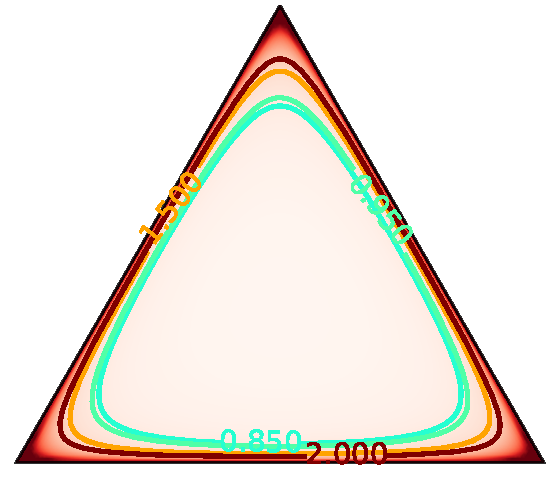
\includegraphics[height=2.14cm]{img/croppedDirichletGraph0.pdf}
        }
        \subfigure[\((0.5,0.5,0.5)\)]{
                \label{fig:subfig:b} %% label for second subfigure b
                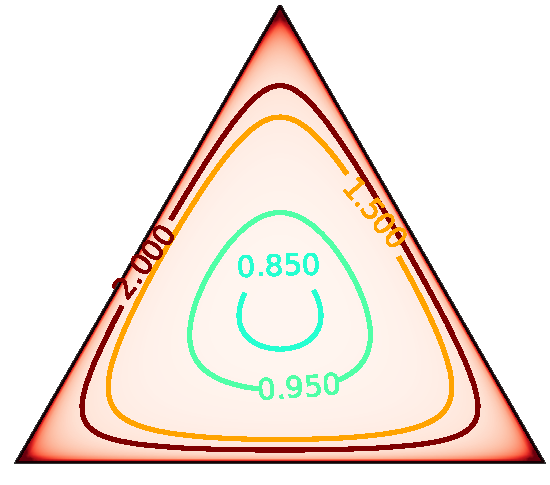
\includegraphics[height=2.14cm]{img/croppedDirichletGraph1.pdf}
        } 
        \subfigure[\((0.25,0.25,0.75)\)]{
                \label{fig:subfig:c} %% label for third subfigure c
                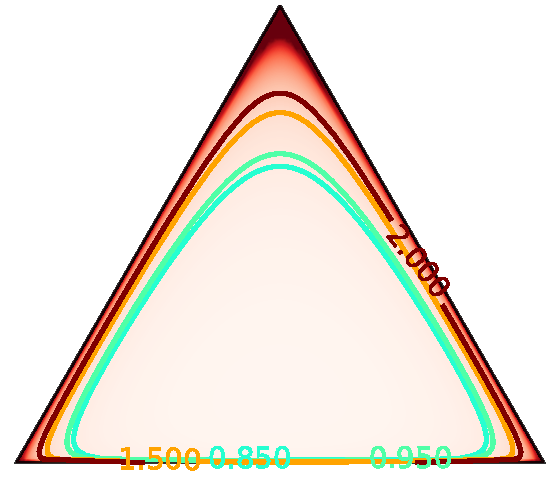
\includegraphics[height=2.14cm]{img/croppedDirichletGraph4.pdf}
        }
        \subfigure[\((0.5,0.5,1.5)\)]{
                \label{fig:subfig:a} %% label for first subfigure d
                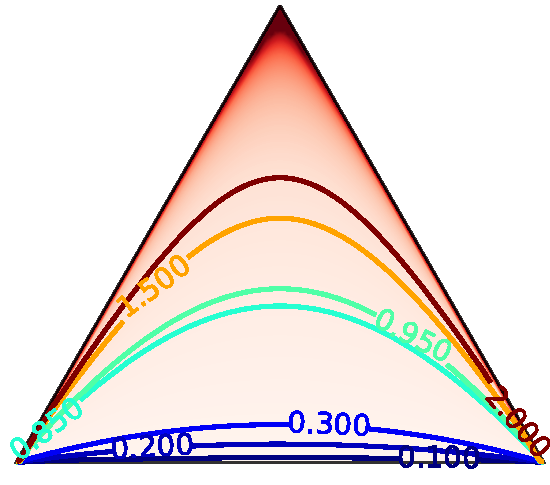
\includegraphics[height=2.14cm]{img/croppedDirichletGraph5.pdf}
        }
        \subfigure[\((0.25,0.75,0.75)\)]{
                \label{fig:subfig:d} %% label for third subfigure e
                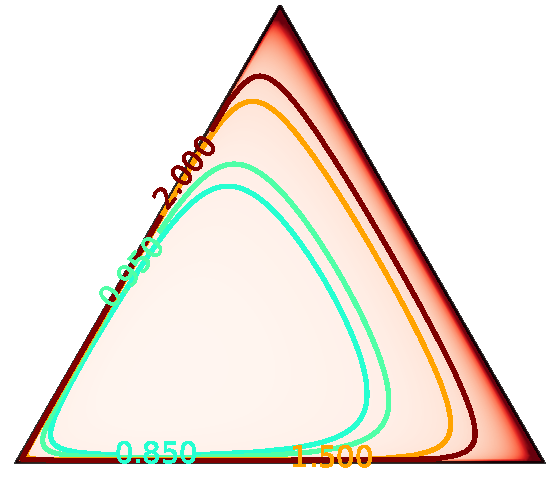
\includegraphics[height=2.14cm]{img/croppedDirichletGraph8.pdf}
        }
        \subfigure[\((0.5,1.5,1.5)\)]{
                \label{fig:subfig:d} %% label for third subfigure f
                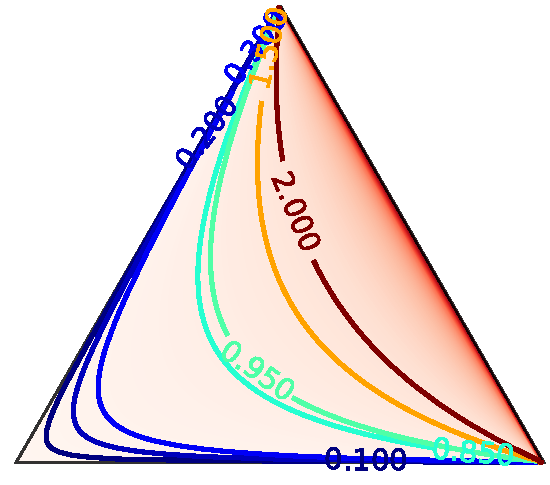
\includegraphics[height=2.14cm]{img/croppedDirichletGraph9.pdf}
        }\hspace{1in}
        \subfigure[\((1.5,1.5,1.5)\)]{
                \label{fig:subfig:d} %% label for third subfigure g
                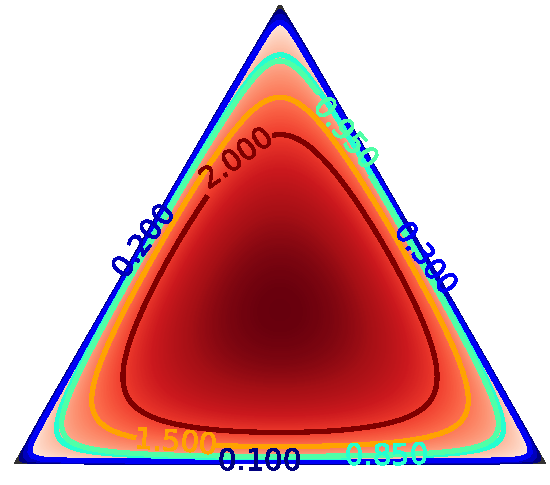
\includegraphics[height=2.14cm]{img/croppedDirichletGraph2.pdf}
        }
        \subfigure[\((2.5,2.5,2.5)\)]{
                \label{fig:subfig:a} %% label for first subfigure h
                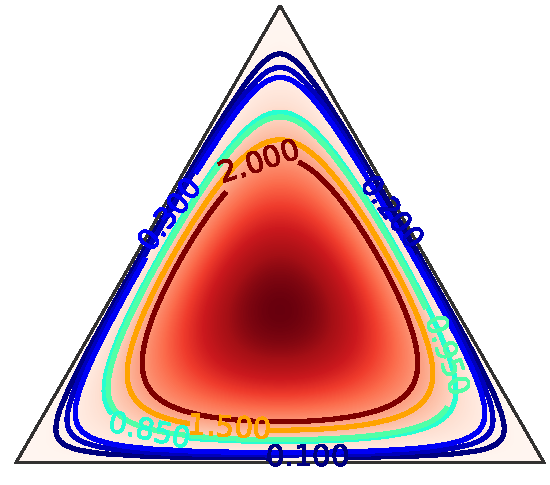
\includegraphics[height=2.14cm]{img/croppedDirichletGraph3.pdf}
        }
        \subfigure[\((1.5,1.5,2.5)\)]{
                \label{fig:subfig:d} %% label for third subfigure i
                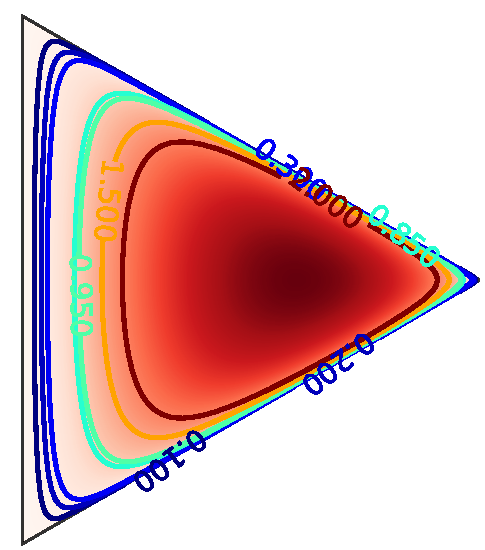
\includegraphics[height=2.14cm]{img/croppedDirichletGraph6.pdf}
        }
        \subfigure[\((2.5,2.5,3.5)\)]{
                \label{fig:subfig:d} %% label for third subfigure j
                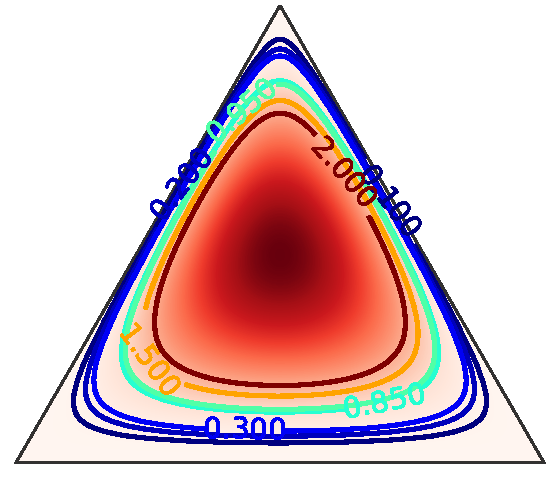
\includegraphics[height=2.14cm]{img/croppedDirichletGraph7.pdf}
        }
        \subfigure[\((1.5,2.5,2.5)\)]{
                \label{fig:subfig:d} %% label for third subfigure k
                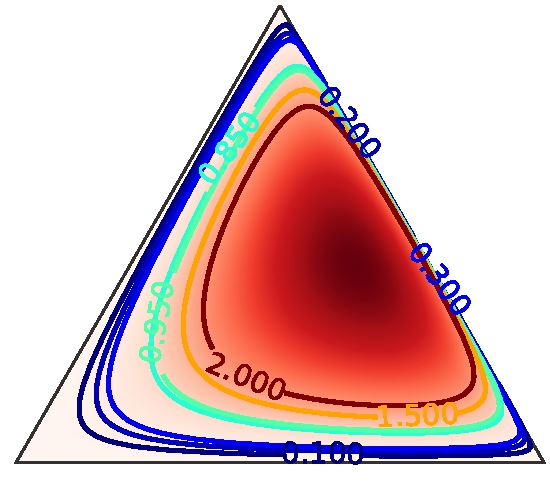
\includegraphics[height=2.14cm]{img/croppedDirichletGraph10.pdf}
        }
        \subfigure[\((2.5,3.5,3.5)\)]{
                \label{fig:subfig:a} %% label for first subfigure l
                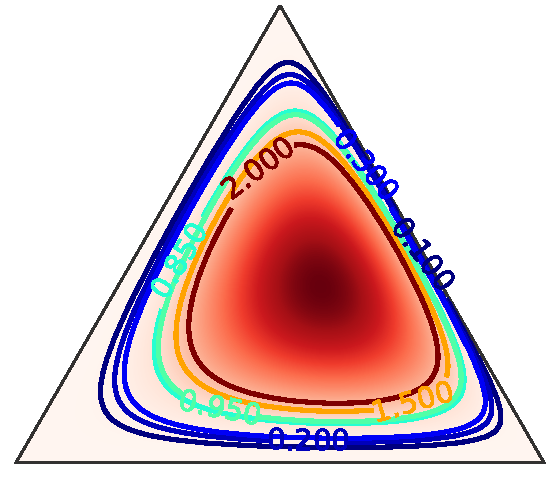
\includegraphics[height=2.14cm]{img/croppedDirichletGraph11.pdf}
        }\hspace{1in}
        \caption{Illustration of Dirichlet distribution's probabilistic density on the 3-dimensional simplex when given different priors. (a,b,g,h) the left four subfigures illustrate the probabilistic density when given the symetric priors for Dirichlet distribution; (c,d,i,j) the central subfigures illustrate the probablistic density given ; (e,f,k,l) }
\end{figure*}
\end{comment}


\section{Proposed Method}
Knowledge base often contains much information about what happened. 
But the exisiting RDF model\cite{klyne2006rdf} on knowledge base lacks the mechanism to maintain the information about what's happening, especially when applied on text stream.  
With the help of knowledge base's structure (detailed in sec \ref{subsec:hs_initialization}), we provide a  lightweight model for organizing the data in knowledge base and the data in text stream simultaneously.

\textit{History state} is the proposed data structure to restore the information about what happened. 
Initially, \textit{history state} extracts category-related history data into a set of tuples, which weighs the importance of given words to the specific category, defined in Definition 1 formally. 
Taking the \textit{military} category in Figure \ref{fig:modelDesc} as an example, the history state of \textit{military} contain the words \textit{army}, \textit{military}, and \textit{shootings} etc. 

\textit{Recent state} is the proposed data structure to maintain the information about what's happening.
It extracts category-related words from incoming text stream, for each time window.
Still taking the \textit{military} category in  Figure \ref{fig:modelDesc} as an example, based on extracted history states, our proposed probabilistic continuous learning model \textsc{HS-Prior-LDA} can recognize the words \textit{libyan} and \textit{rebel} in the time window 2011-07-28 in the text stream are related to the category \textit{military}. 
Furthermore the time series analysis on the neighboring recent states can recognize the set of events' candidate words, and finally detects the events in the text stream. 
In the example of Figure \ref{fig:modelDesc}, the words \textit{libyan} and \textit{rebel} are related to the \textit{military} event ``\#libya Libyan rebels chief is killed (2011-07-28)''.

After processing each time window's data, the history states can be incrementally updated by the recent state. 
In this way, the proposed model utilizes the rich history data in knowledge base, and performes continous learning on the incoming text stream, which can promote the accuracy of event detection significantly. 
The followings definitions are the concepts used by the continous learning model \textsc{HS-Detector}. 


\begin{rmk}[History State] 
The history state of the specific category is defined by a set of tuples, in which the first element is the word \(w^{(c)}_i\) related to the category \(c\), and the second element is the chi-square score \(chi(c,w^{(c)}_{i})\) under the category \(c\). 
And we denote the history states of category \(c\) as \(\bm{h}_c=\{<w^{(c)}_i,chi(c,w^{(c)}_{i})>\}_{i=1,...,N_c}\).
\end{rmk}

\begin{rmk}[Recent State] 
The recent state at time \(t\) of the specific category \(c\) is defined by a set of tuples, and detenoted as \(\bm{r}_{c,t}=\{<w^{(c)}_i,n(c,t,w^{(c)}_{i})>\}_{i=1,...,N_c}\), in which word \(w^{(c)}_{i}\) is related to the category \(c\), and \(n(c,t,w^{(c)}_{i})\) is its document frequency in the time window \(t\).
\end{rmk}


\begin{rmk}[The Set of Events' Candidate Words] 
The set of events' candidate words \(\mathcal{B}_{c,t}\) are defined by the bursty words in recent state \(\bm{r}_{c,t}\).
\end{rmk}

\begin{rmk}[Event Phrase] 
Event phrase \(\mathcal{C}_{c,t,i}\) is the \(i\)-th combination of words which occured in the set of events' cadidate words \(\mathcal{B}_{c,t}\), and represents the \(i\)-th event happend in time \(t\) under the category \(c\).
\end{rmk}

\begin{rmk}[Event Related Articles] Event related articles \(\mathcal{D}_{c,t,i}\) are articles that relate to the \(i\)-th event in time \(t\) under the category \(c\), and correspond to the event phrase \(\mathcal{C}_{c,t,i}\).
\end{rmk}

Section \ref{subsec:hs_initialization} explains the details of how to initialize history states from knowledge base.
Section \ref{subsec:rs_initialization} shows how to perform continous learning for updating history states and recent states.
And section \ref{subsec:detection} interprets the high accuracy event detection based on the processed recent states.

\begin{table}
\scriptsize
\caption{Notations used by \textsc{NSDetector}}
\label{tbl:notations}
\begin{tabular}{|c|p{0.06\columnwidth}|p{0.66\columnwidth}|} \hline
%first part: normalization initialization
\multirow{5}{0.13\columnwidth}{History States' Initialization} & \(G^{(0)}\) & Taxonomy's Graph in Knowledge Base\\ \cline{2-3}
& \(G^{(1)}\) & Category-Page Bipartite Graph in Knowledge Base\\ \cline{2-3}
& \(G^{(2)}\) & Page-Content Map in Knowledge Base\\ \cline{2-3}
& \(c\) & topic related category node in \(G^{(0)}\), \(G^{(1)}\) \\ \cline{2-3}
& \(K_{\bm{KB}}\) & number of pre-defined topics in Knowledge Base \\ \cline{2-3}
& \(h_{c,w}\) & word \(w\)'s history state (chi-square score) in category \(c\) \\ \hline
%second part: normalization maintenance
\multirow{4}{0.13\columnwidth}{Normal States Maintenance} & \(\lambda\) & normal state weight in  NS-Prior-LDA\\ \cline{2-3}
& \(\tau_{c,w}\) & word \(w\)'s prior knowledge confidence for topic \(c\) in NS-Prior-LDA\\ \cline{2-3}
& \(S_c\) & topic \(c\)'s all normal states related words \\ \cline{2-3}
& \(K\) & number of topics in NS-Prior-LDA such as \(K>K_{\bm{KB}}\)\\ \hline
%third part: event detection
\multirow{5}{0.13\columnwidth}{Event Detection} & \(\mathcal{B}_{c, t}\)  & event words set detected from topic \(c\) at time \(t\)  \\ \cline{2-3}
& \(\mathcal{G}_{c, t}\)  & hot word graph constructed from \(\mathcal{B}_{c, t}\) \\ \cline{2-3}
& \(\mathcal{C}_{c,t,i}\) & event \(i\)-th related words in topic \(c\) at time \(t\) \\ \cline{2-3}
& \(\mathcal{D}_{c,t,i}\) & event \(i\)-th related articles in topic \(c\) at time \(t\) \\ \cline{2-3}
& \(\rho\) & density threshold for the sub-graph constructed by event words  \\ \hline

\end{tabular}
\label{symbolsInModel}
\end{table}


\subsection{History States Initialization}\label{subsec:hs_initialization}
In this part, we discuss in detail how to initialize the normal states from the given knowledge base. 
The knowledge base such as Wikipedia has the structure of classes, subclasses, instances, and the edges between them. 
This structure usually can be represented as triples in RDF graph\cite{klyne2006rdf}, which is adopted to build DBPedia\cite{auer2007dbpedia} and YAGO\cite{suchanek2007yago} from Wikipedia. 
%但是,往往在图上的计算是非常费时的。
%But The RDF and other methods often 

\textbf{Taxonomy Graph \(G^{(0)}\)}. The directed edges in \(G^{(0)}\) represent the class-subclass relations in the knowledge base. 
Taking Wikipedia for example (Figure \ref{fig:NSinitializaton}), the node \textit{Main topic classifications}\footnote{\url{https://en.wikipedia.org/wiki/Category:Main_topic_classifications}} has the subclass \textit{Society}, further contains the subclass \textit{Politics}, which is the ancestor of the subclass \textit{Military}.

\textbf{Category-Page Bipartite Graph \(G^{(1)}\)}. 

\textbf{Page-Content Maps \(G^{(2)}\)}.

As \(G^{(0)}\) is not a Directed Acyclic Graph originally\cite{faralli2015large}, we need to remove the , PageRank-HITS\cite{Yan:2015wq}. 



\begin{algorithm}
\scriptsize
\caption{Normal States Initialization from Knowledge Base}
\label{alg:normalStatesInit}

\KwIn{Taxonomy's Graph \(G^{(0)}\), Category-Page Bipartite Graph \(G^{(1)}\), Page-Content Bipartite Graph \(G^{(2)}\), topic related category node \(c\)}
\KwOut{Normal states \(\bm{f}_c\) on topic \(c\)}
\(Pages(c)\leftarrow \varnothing\)\\
DAG \(G^{(0)'} \leftarrow\) Remove Cycles of \(G^{(0)}\) by nodes' HITS-PageRank scores. \\
\(SuccessorNodes(c) \leftarrow \) Breadth-first-traverse(\(G^{(0)},c\))\\
\For{\(node \in SuccessorNodes(c)\)}{
    \(Pages(c) \leftarrow Pages(c) \cup G^{(1)}.neighbours(node)\)\\
}
\(WordFrequencyTable(c) \leftarrow \) do word count on the text contents of \(Pages(c)\) \\
\(WordFrequencyTable(All) \leftarrow \) do word count on the text contents of all pages in \(G^{(2)}\).\\
\For{word \(w\) in WordFrequencyTable(All).keys()}{
    \(\tau_{c,w} \leftarrow \) \(w\)'s chi-square score on \(WordFrequencyTable(c)\) and \(WordFrequencyTable(All)\).
}
\Return{\(\bm{f}_c\)}
\end{algorithm}


%TODO

\begin{figure}
    \centering
    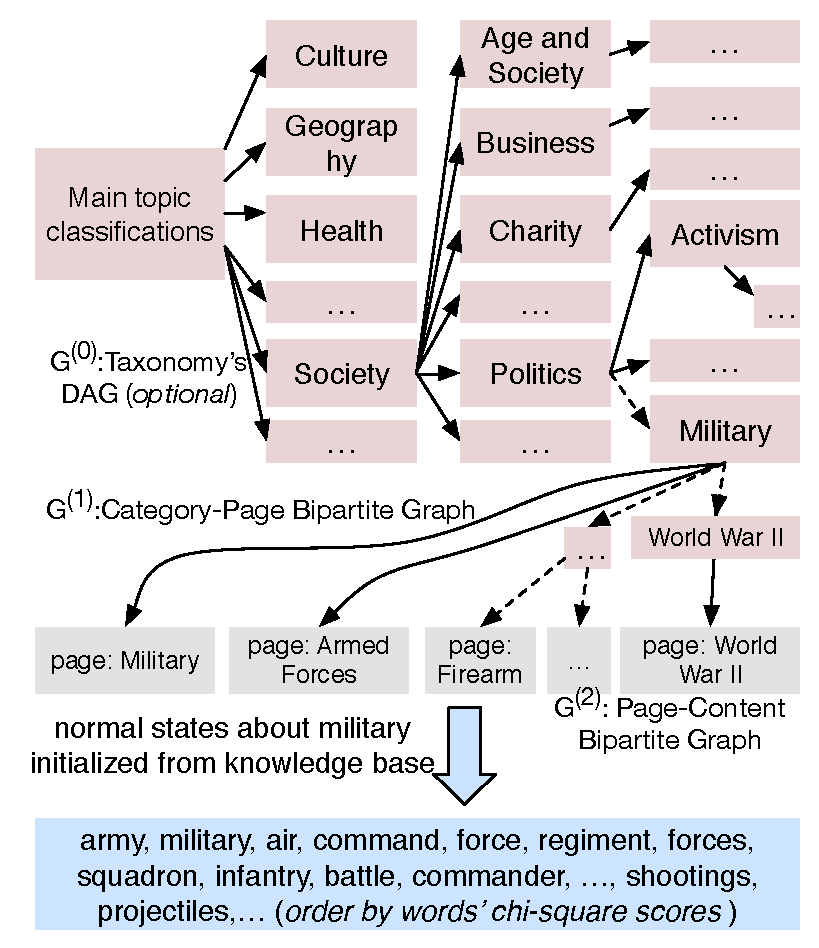
\includegraphics[width=.85\columnwidth]{img/initializationExample.pdf}  
    \caption{Illustration on how to initialize normal states from wikipedia (an example on the initialization of the normal states about \textit{military}).}
    \label{fig:NSinitializaton}
\end{figure}




\subsection{Recent States' Maintenance}
\label{subsec:rs_initialization}

\begin{comment}
\begin{figure}[t]
    \centering
    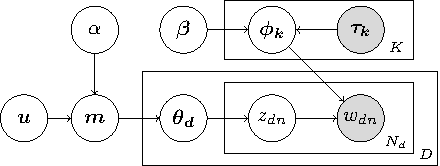
\includegraphics[width=0.75\columnwidth]{model/lda_tikz.pdf}
    \caption{Probabilistic model for training normal states by using history information.}
    %The convolution neural network for extracting character-level representations of words. Dashed arrows indicate a dropout layer applied before character embeddings are input to CNN.}
    \label{fig:NS-Prior-LDA}
\end{figure}
\end{comment}

\ \ Our topic modeling, want to learn the first \(k\) topics with Wikipedia Article \(k\) topics as close as possible, and we will be Wikipedia article \(k\) before 1000 words) was added to the theme of the word frequency word in the subject a priori distribution on the.
Learning to be the first \(k\) Subject polynomial distribution of the word, referred to as \(\phi_k \), Wikipedia article \(k \) distribution of topics for \(\tau_k \), then this formalized process is expressed as: \(\ \phi_k \sim Dir(\beta + \tau_k) \).
Formal presentation of the explanation is: With prior knowledge \(\tau_k \) after the theme \(\phi_k \) is no longer simply rely on symmetric priori \(\beta \), different words right is not the same weight , such as a discussion of "fashion" theme in Wikipedia, it will refer to "dress", "grand", "blue", "gold" and other words, with the asymmetric priori \(\beta + \tau_k \) after in microblogging "fashion" theme "dress" the proportion will be increased in this way so that microblogging corpus theme tends to Wikipedia topic.
\(\tau_k \) in the first \(v \) words such as formula (\ref{eq:wikiPrior}).
Where \(S_k \) as a set of candidate words: high-quality information to use Wikipedia, we extract the theme \(\phi_k \ \) in the higher-word word frequency candidate set \(S_k \).
We can control set \(S_k \) in size, the size of the control is usually set for 1000.
The number of frequency \(n_{kv} \) for the word \(v \) (\ k) appears in the Wikipedia article themes.
If the word \(v \) does not appear in the candidate set \(S_k \), and then set a priori knowledge \(\tau_{kv} = 0 \), otherwise, the word frequency is proportional to \(n_{kv} \) with the prior knowledge of weight \(W\).
In the latter experiment, we will be on a priori knowledge of weights \(W \) will be discussed. 

\begin{table}[!htbp]
\begin{tabular}{l}
1. Draw corpus prior distribution \(\bm{m} \sim Dir(\alpha \bm{u})\), where \(\bm{u}\)\\
 \ \ \ \ is the uniform distribution. \\
2. For each topic \(k \in \{1,\cdots,K\}\),\\
\ \ \ \ (a) word distribution on the topic \(\bm{\phi_k} \sim Dir(\bm{\beta}+ \bm{\tau_k})\). \\
    
3. For each document index \(d \in \{1,...,D\}\), \\
\ \ \ \ (a) topic distribution on the document \(\theta_d \sim Dir(\bm{m})\), \\
\ \ \ \ (b) for each word index \(n \in \{1,\cdots,N_d\}\),\\
\ \ \ \ \ \ \ \ i. word's topic assignment \(z_{dn} \sim Multinomial(\theta_d)\), \\
\ \ \ \ \ \ \ \ ii. word \(w_{dn} \sim Multinomial(\phi_{z_{dn}})\). \\
\end{tabular}
\end{table}

\begin{scriptsize}
\begin{equation}
\label{eq:wikiPrior}
\begin{aligned}
\tau_{kv}=
\left\{ \begin{aligned}
\lambda \frac{f_{kv}}{\sum_{v\in S_{kv}}f_{kv}} &,v\in S_{k}\ and  \ k \leq K_{\bm{KB}} \\
0&,v \notin S_{k} \ or \ k > K_{\bm{KB}} \\
\end{aligned}\right.
\end{aligned}
\end{equation}
\end{scriptsize}

\begin{scriptsize}
\begin{equation}
\label{eq:initProbability}
\begin{aligned}
\hat{q}_{k|v}=
\left\{ \begin{aligned}
\frac{\tau_{kv}}{\sum_{k=1}^{K}\tau_{kv}} &,\sum_{k}\tau_{kv}>0 \\
0&, \sum_{k}\tau_{kv}=0 \ and \ k \leq K_{\bm{KB}} \\
1/(K-K_{\bm{KB}})&,\sum_{k}\tau_{kv}=0 \ and \ k > K_{\bm{KB}}
\end{aligned}\right.
\end{aligned}
\end{equation}
\end{scriptsize}

\begin{scriptsize}
\begin{equation}
\label{eq:KBPriorLDAgibbs}
\begin{aligned}
&p(z_{dn}=k|w_{dn}=v,z_{\neg{dn}},w_{\neg{dn}},\alpha\bm{m},\beta,\tau)\\
&\ \ \propto (n^{(d)}_{dk}+\alpha m_k)\frac{n^{(w)}_{kv}+\tau_{kv}+\beta}{n^{(w)}_{k,.}+\tau_{k,.}+V\beta}
\end{aligned}
\end{equation}
\end{scriptsize}

\begin{algorithm}
\scriptsize
\caption{NS-Prior-LDA Learning Algorithm}
\label{alg:gibbsSamplingKBPriorLDA}
\KwIn{Documents \(\mathcal{D}\) (a.k.a., \(\bm{w_{1:D}}\)), and normal states \(\bm{f}_{1:K_{\bm{KB}}}\)}
\KwOut{The sufficient statistics \(\bm{n^{(d)}}\), \(\bm{n^{(w)}}\)}
\tcc{Initialization of NS-Prior-LDA}
\For{\(d=1:D\)}{
    \For{\(n=1:N_d\)}{
        \(v=w_{dn}\), sample \(z_{dn}=k\) as Eq(\ref{eq:wikiPrior})(\ref{eq:initProbability}).\\
        Update the sufficient statistics \(n^{(d)}_{d,k}\), \(n^{(w)}_{k,v}\).\\
            }
        }
\For{\(i= 1:I\)}{
    \tcc{E-Step of NS-Prior-LDA}
    \For{\(i=1:I_E\)}{
        \For{\(d=1:D\)}{
            \For{\(n=1:N_d\)}{
                Set \(v=w_{dn}\), and reset the sufficient statistics \(n^{(d)}_{d,z_{dn}}\), \(n^{(w)}_{z_{dn},v}\).\\
                Resample \(z_{dn}=k\) as Eq(\ref{eq:wikiPrior})(\ref{eq:KBPriorLDAgibbs}).\\
                Update the sufficient statistics \(n^{(d)}_{d,k}\), \(n^{(w)}_{k,v}\).\\
            }
        }
    }
    \tcc{M-Step of NS-Prior-LDA}
    Optimize \(\alpha \bm{m}\) by the fixed-point iteration\cite{wallach2008structured}. 
}
\Return{\(\bm{n^{(w)}}\)}
\end{algorithm}

The line 12 in Algorithm \ref{alg:gibbsSamplingKBPriorLDA} is implemented according to \cite{wallach2008structured}\footnote{\url{https://github.com/mimno/Mallet/blob/master/src/cc/mallet/types/Dirichlet.java}}, which can optimize \(\alpha \bm{m}\) for promoting NS-Prior-LDA's fitting to documents \(\mathcal{D}\). 

\subsection{Detecting Events from Recent States}
\label{subsec:detection}
The state of attention of social issue k at time t in cyberspace is binary, namely at the peak or not at the peak. We denote it by hidden binary variable \(s_{k,t}\), which is 1 or 0. We do the inference for the hidden variable \(s_{k,t}\) according to Poisson distribution according to Reference\cite{Diao:2012wj} 10,11. If the state of attention of social issue k at time t is "not at peak", then the probability density function is 
\(p(x_{k,t}|s_{k,t}=0)=e^{-\mu_0 }  \frac{\mu_0^{x_{k,t}}}{x_{k,t}!}\) otherwise the probability density function is \(p(x_{k,t}|s_{k,t}=0)=e^{-\mu_1 }  \frac{\mu_1^{x_{k,t}}}{x_{k,t}!}\)
In the above functions the symbol \(x_{k,t}\) denotes the attention of social issue \(k\) at time \(t\) , the symbol A denotes the constant, \(\mu_0\) and \(\mu_1\) represent the average of \(x_{k,t}\) at peak and not at peak respectively. The state \(s_{k,t}\) is inferred from \(ratio=\frac{p(x_{k,t} |s_{k,t}=0)}{p(x_{k,t} |s_{k,t}=1)} \).
In calculation, we use the log ratio to determine whether the attention is at peak as in equation (\ref{eq:logratio}). \(\log ratio>0 \) indicates that the attention of social issue \(k\) at time \(t\) is not at peak, otherwise at peak. 
\begin{equation}
\label{eq:logratio}
\log ratio=-(\mu_0-\mu_1 )+x_{k,t}(\log \mu_0 -\log⁡ \mu_1)
\end{equation}

\begin{algorithm}
\scriptsize
\label{alg:eventKeywordsSearchMethod}
\caption{Spectral Clustering Based Event Phrase Extraction}
\label{alg:eventKeywordsSearchMethod}
\KwIn{\(\mathcal{B}_{k,t},\mathcal{G}_{k,t},\rho\)}
\KwOut{\(\mathcal{C}_{k,t}\)}
\(n_{k,t}\)=number of connected component in \(\mathcal{G}_{k,t}\)\\
\For{\(n \in \{ n_{k,t}, \cdots, |\mathcal{G}_{k,t}|\}\) }{
    \(\mathcal{C}_{k,t}=SpectralClustering(\mathcal{G}_{k,t},n)\)\\
    \If{\(min_{i\in \{1,\cdots,n\}} Density(\mathcal{C}_{k,t,i},\mathcal{G}_{k,t})>\rho\)}{
        return \(\mathcal{C}_{k,t}\)
    }
}
\end{algorithm}

\begin{comment}
\begin{figure}
\centering
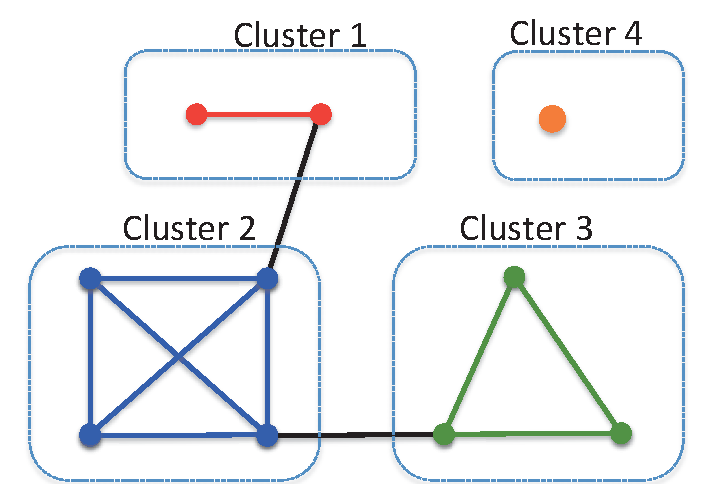
\includegraphics[height=3cm]{img/wordClusterGraph.eps}
%todo
\caption{Hot words between the heat pattern forming word time window edge weight calculated by the PMI obtained between words, to obtain spectral clustering clustering clustering}
\label{fig: windowsBurstyWordGraph}
\end{figure}
\end{comment}
\textbf{event} phrase Mining
% Refer to bursty.py
\ \ Microblogging mining events can be represented by a variety of ways, a single word, phrase, or topic.
Here we use the form of phrase, said event.
In this paper, the phrase indicates that the event is due to the fact that: the same period of time when there are multiple areas of internal hot words appear, a collection of hot words \(\mathcal{B}_{k, t} \) between the hot words great probability is interrelated. For example, observed "mac", "os", "lion" three words are in a state of emergency.
In fact, the state of emergency three words is to publish a new system "mac os lion" event caused by Apple, in order to find the association between words and events, we use spectral clustering based search methods.

As shown in Figure \ref{fig: windowsBurstyWordGraph} below, we will one area, a hot word of the time window and hot words between to diagram.
Hot words set \(\mathcal{B}_{k, t} \) formed in FIG using \textbf{hot word graph} \(\mathcal{G}_{k, t} = (\mathcal{B}_{k, t}, \mathcal{E}_{k, t}) \) indicates,
\(\mathcal{E}_{k, t} = \{(a, b) | a \in \mathcal{B}_{k, t}, b \in \mathcal{B}_{k, t }, PMI (\mathcal{D}_{k, t}, a, b)> 0 \} \), where \(PMI (\mathcal{D}_{k, t}, a, b) \) the field \(k \) time window \(t \) related microblog \(\mathcal{D}_{k, t} \) on the word \(a\) and the word \(b\) point metric information between each other.
% Refer to bursty.py getSimGraph () function

Given a field \(k\) and the time window \(t\), in which the number of events can not be determined in advance.
The two most extreme situations are: events coarse granularity, said the event is equal to the number of Figure \(\mathcal{G}_{k, t} \) in the number of connected components; events finer granularity display, event number equal to \(\mathcal{G}_{k, t} \) the number of points.
To do this, we use the Density to the degree of density of quantum graphs \(2 \#Edge / (\# Node \ cdot (\# Node-1)) \), the more the greater if the edge density in the range of Density in \((0,1] \).
Density can be a good indicator to determine the size indicates the event: too many unrelated phrases to put together an event can not be represented, too fine particle size, such as a single word can represent only part of the event; only in close co-occurrence of the phrase to a reasonable It indicates that the event granularity.
To this end, we have designed events phrase search algorithm \ref{alg:eventKeywordsSearchMethod}: We try to find a reasonable number of spectral clustering Clustering \(n \), let \(n \) from a smaller value ( event corresponds to coarser granularity representation) to start the search, then the most likely cluster cluster size is too large, its performance is the clustering results in one or more small Density indicators; continue to increase the number of clusters \(n \), the event represents reduced size, reduced the size of clusters of clusters, thus making the Density index increases; when all cluster clustering Density indicators are larger than the threshold \(\tau \), the search terminates, returning clustering results \(\mathcal{C}_{k, t}\).
As the above process algorithm \ref{alg:eventKeywordsSearchMethod} description line 2 to line 5, we use in practice \(\rho = 0.6 \).
We call \(\mathcal{C}_{k, t} \) results in each cluster to cluster \textbf{event} phrase.

\textbf{detected events related to micro-blog}
\ \
By algorithm \ref{alg:eventKeywordsSearchMethod} find art \(k \) time window \ \(t \) within the \(| \mathcal{C}_{k, t} | \) events phrase later, you can also further find each event and the corresponding event phrase microblogging.
We looked at the first \(i \) events phrase \(\mathcal{C}_{k, t, i} \),
The phrase based on the number of elements distinguish the event, there are three situations: (1) the phrase event more than two hot words, he said while the event is not a phrase between any two words We have a very strong relationship between the co-occurrence, so just pay attention to the co-occurrence relationship stronger side; (2) event phrase has two hot words; (3) the event is only a hot word in the phrase.
Weibo text length is shorter, not all of the microblogging event will include the phrase \(\mathcal{C}_{k, t, i} \) in all the words.
Such as those on "Apple released the new system mac os lion" event, the event phrase "mac", "os", "lion" does not need to appear in all of the micro-Bo, just check the co-occurrence of a strong relationship between the two words appear together whether in an article in the field \(k \) time window \(t \) micro-Bo: If there is, then added to the events related to the collection \(\mathcal{D}_{k, t, i} \) in.
For the case of a third cluster cluster contains only a hot word, we only need to identify areas \(k \) contains the hot word of all micro-blog, and add the event to the relevant set \(\mathcal{D}_{k, t, i} \) in.
Ultimately, we can get the field \(k \) next time window \(t \) in the event the phrase relating to events microblogging \(\{(\mathcal{C}_{k, t, i}, \mathcal{D}_{k, t, i}) \}_{i=1}^{| \mathcal{C}_{k, t} |} \).

\section{Experiments}
\subsection{Effects of Normal States}
We use 20newsgroups\cite{lang1995newsweeder} dataset\footnote{http://qwone.com/~jason/20Newsgroups} to check the effects of normal states initialization.

\begin{comment}
\begin{table}[]
\scriptsize
\centering
\caption{Normal State's cateogries corresponding to the 20-newsgroups corpus, and the F1 score on the classification task}
\label{my-label}
\begin{tabular}{|l|l|}
\hline
comp.graphics            & Computer graphics      \\ \hline
comp.os.ms-windows.misc  & Microsoft Windows      \\ \hline
comp.sys.ibm.pc.hardware & IBM personal computers \\ \hline
comp.sys.mac.hardware    & Macintosh computers    \\ \hline
comp.windows.x           & X Window System        \\ \hline
rec.autos                & Automobiles            \\ \hline
rec.motorcycles          & Motorcycles            \\ \hline
rec.sport.baseball       & Baseball               \\ \hline
rec.sport.hockey         & Hockey                 \\ \hline
sci.crypt                & Cryptography           \\ \hline
sci.electronics          & Electronics            \\ \hline
sci.med                  & Medicine               \\ \hline
sci.space                & Outer space            \\ \hline
misc.forsale             & Sales                  \\ \hline
talk.politics.misc       & Politics               \\ \hline
talk.politics.guns       & Gun politics          \\ \hline
talk.politics.mideast    & Middle East           \\ \hline
talk.religion.misc       & Religion               \\ \hline
alt.atheism              & Atheism                \\ \hline
soc.religion.christian   & Christians             \\ \Xhline{3\arrayrulewidth}
LDA & 0.74\\ \hline
BOW & 0.84\\ \hline
doc2vec & 0.73\\ \hline
NS-Prior-LDA & 0.89\\ \hline
\end{tabular}
\end{table}
\end{comment}

\begin{table}[]
\tiny
\centering
\caption{My caption}
\label{my-label}
\begin{tabular}{|l|l|l|l|l|l|}
\hline
 &  & LDA & BOW & doc2vec & \begin{tabular}[c]{@{}l@{}}NS-Prior-\\ LDA\end{tabular} \\ \hline
comp.graphics & Computer graphics &  &  &  &  \\ \hline
comp.os.ms-windows.misc & Microsoft Windows &  &  &  &  \\ \hline
comp.sys.ibm.pc.hardware & IBM personal computers &  &  &  &  \\ \hline
comp.sys.mac.hardware & Macintosh computers &  &  &  &  \\ \hline
comp.windows.x & X Window System &  &  &  &  \\ \hline
rec.autos & Automobiles &  &  &  &  \\ \hline
rec.motorcycles & Motorcycles &  &  &  &  \\ \hline
rec.sport.baseball & Baseball &  &  &  &  \\ \hline
rec.sport.hockey & Hockey &  &  &  &  \\ \hline
sci.crypt & Cryptography &  &  &  &  \\ \hline
sci.electronics & Electronics &  &  &  &  \\ \hline
sci.med & Medicine &  &  &  &  \\ \hline
sci.space & Outer space &  &  &  &  \\ \hline
misc.forsale & Sales &  &  &  &  \\ \hline
talk.politics.misc & Politics &  &  &  &  \\ \hline
talk.politics.guns & Gun politics &  &  &  &  \\ \hline
talk.politics.mideast & Middle East &  &  &  &  \\ \hline
talk.religion.misc & Religion &  &  &  &  \\ \hline
alt.atheism & Atheism &  &  &  &  \\ \hline
soc.religion.christian & Christians &  &  &  &  \\ \hline
In total & &  &  &  & \\ \hline
\end{tabular}
\end{table}

\begin{figure}
        \centering
        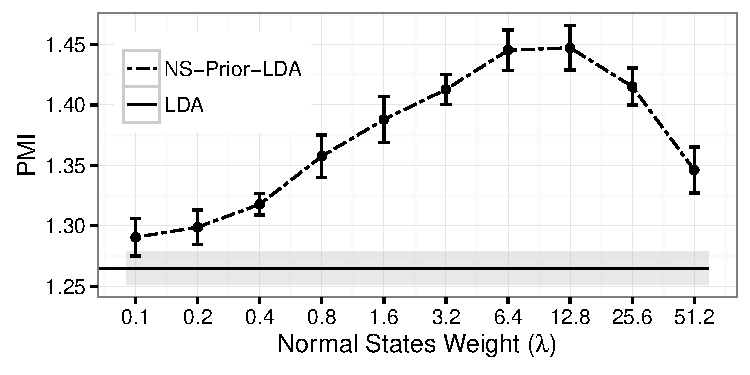
\includegraphics[height=4.0cm]{img/pmi.pdf}
        \caption{The quality of all twitter topics learned by NS-Prior-LDA increases with normal states weight (\(\lambda\)) before \(\lambda=12.8\). The optimized PMI is gained with moderate normal states weight when considering topics \(k\leq K_{\bm{KB}}\) and topics \(k > K_{\bm{KB}}\) together.}
\end{figure}

\begin{comment}
\begin{figure}
        \centering
        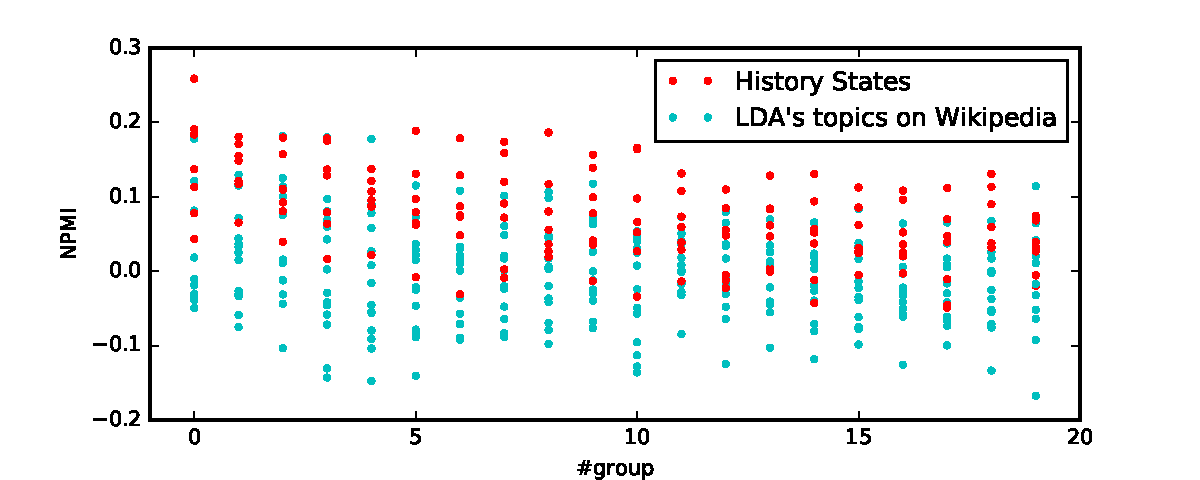
\includegraphics[width=1.0\columnwidth]{img/NPMI.pdf}
        \caption{The comparison on NPMI\cite{Aletras2013EvaluatingTC}\cite{Rder2015ExploringTS} between LDA's topics and normal states initialized from Wikipedia}
\end{figure}
\end{comment}



\begin{table}
\centering
\caption{The PMI of twitter topics learned by NS-Prior-LDA, its variant, and other baselines}
    \begin{tabular}{|l|l|c|}
    \hline
    Model & Prior Knowledge & PMI \\ \hline
    LDA & None  & 1.265 \(\pm\) 0.013     \\ \hline
    BBTM\cite{Yan:2015wm} & None    & 1.467 \(\pm\) 0.017     \\ \hline
    NS-Prior-LDA\(^{(-)}\)   &   \begin{tabular}[c]{@{}l@{}}\footnotesize{Words in categories simply}\\ \footnotesize{extracted from Wikipedia}\end{tabular} & 1.439 \(\pm\) 0.010     \\ \hline
    NS-Prior-LDA         & \begin{tabular}[c]{@{}l@{}}\footnotesize{Normal states initialized} \\\footnotesize{from wikipedia}\end{tabular} & 1.523 \(\pm\) 0.017     \\ \hline
    \end{tabular}
\label{tbl:NS-Prior-LDA}
\end{table}

\begin{table*}[ht]
\centering
\caption{Normal States initialized from Wikipedia and topical words learned from NS-Prior-LDA}
\label{my-label}
\scalebox{0.88}{
\begin{tabular}{|cc|cc|cc|cc|cc|cc|}
\hline
\multicolumn{2}{|c|}{\textit{Aviation}} & \multicolumn{2}{c|}{\textit{Health}} & \multicolumn{2}{c|}{\textit{Middle East}} & \multicolumn{2}{c|}{\textit{Military}} & \multicolumn{2}{c|}{\textit{Mobile Phones}} & \multicolumn{2}{c|}{\textit{Video Games}} \\
\begin{tabular}[c]{@{}c@{}}Normal\\ States\end{tabular} & \begin{tabular}[c]{@{}c@{}}Topical\\ Words\end{tabular} & \begin{tabular}[c]{@{}c@{}}Normal\\ States\end{tabular} & \begin{tabular}[c]{@{}c@{}}Topical\\ Words\end{tabular} & \begin{tabular}[c]{@{}c@{}}Normal\\ States\end{tabular} & \begin{tabular}[c]{@{}c@{}}Topical\\ Words\end{tabular} & \begin{tabular}[c]{@{}c@{}}Normal\\ States\end{tabular} & \begin{tabular}[c]{@{}c@{}}Topical\\ Words\end{tabular} & \begin{tabular}[c]{@{}c@{}}Normal\\ States\end{tabular} & \begin{tabular}[c]{@{}c@{}}Topical\\ Words\end{tabular} & \begin{tabular}[c]{@{}c@{}}Normal\\ States\end{tabular} & \begin{tabular}[c]{@{}c@{}}Topical\\ Words\end{tabular} \\ 
\hline
aircraft & air\scriptsize(3253) & health & weight\scriptsize(16344) & al & \textcolor{red}{\textit{\#syria}}\scriptsize(4212) & army & killed\scriptsize(4055)  & android & iphone\scriptsize (13674) & game & games\scriptsize(8812) \\ 
air & plane & patients & loss & israel & \textcolor{red}{\textit{\#bahrain}} & military & news & mobile & apple & player & liked \\ 
airport & flight & medical & diet & iran & people & air & \textcolor{red}{\textit{\#libya}}\scriptsize(3503) & nokia & android & playstation & free \\ 
flight & time & disease & health & arab & israel & command & libya & ios & app & gameplay & xbox \\
airline & airlines & treatment & cancer & israeli & police & force & rebels & phone & ipad & nintendo & 360 \\
airlines & news & hospital & lose & egypt & \textcolor{red}{\textit{\#libya}}\scriptsize(2557) & regiment & people & samsung & samsung & games & playing \\
aviation & boat & patient & fat & egyptian & \#egypt & forces & police & game & mobile & players & played \\
flying & airport & clinical & tips & ibn & news & squadron & war & app & blackberry & xbox &iphone\scriptsize(2820)\\
pilot & force & symptoms & treatment & jerusalem & \#israel & infantry & libyan & iphone & tablet & mode & time\\
squadron & fly & cancer & body & syria & world & battle & attack & htc & apps & arcade & \textcolor{red}{\textit{ps3}}\\
flights & hurricane & cells & healthy & iraq & syria & commander & u.s. & smartphone & free & wii & trailer\\
pilots & navy & blood & study & palestinian & protest & ship & gaddafi & phones & \#android & multiplayer & online\\
raf & flying & therapy & pain & syrian & israeli & corps & army & blackberry & htc & sega & hours\\
airways & aircraft & drug & exercise & iranian & egypt & navy & forces & apps & google & console & ipad\\
fighter & \textcolor{red}{\textit{irene}} & medicine & \#health & ottoman & al & brigade & pakistan & ipad & galaxy & enemies & app\\
boeing & crew & brain & natural & islamic & syrian & battalion & afghanistan & gsm & ios & characters & player\\
runway & sky & care & disease & iraqi & protesters & lieutenant & military & lte & store & playable & wii\\
force & crash & syndrome & acne & abu & arab & aircraft & attacks & symbian & windows & character & ops\\
crashed & jet & infection & hair & jewish & rights & officer & troops & devices & mac & video & download\\
flew & pilot & disorder & surgery & persian & libya & naval & dead & smartphones & phones & graphics & nintendo\\
\hline
\end{tabular}
}
\end{table*}



\begin{table}

\scriptsize
\centering
\caption{Normal States initialized from Wikipedia and topical words learned from NS-Prior-LDA}
\scalebox{0.95}{
    \begin{tabular}{|l|l|l|l|l|}
    \hline
    Method & \begin{tabular}[c]{@{}l@{}}Recall@ \\ Benchmark1\end{tabular} & \begin{tabular}[c]{@{}l@{}}Precision@ \\ Benchmark2\end{tabular} & \begin{tabular}[c]{@{}l@{}}Recall@ \\ Benchmark2\end{tabular} & \begin{tabular}[c]{@{}l@{}}DERate\\(Duplicate \\ Event Rate)\end{tabular} \\ \hline
    UMass System\cite{Allan:2000wu} & 0.882 & 0.138 & 0.941 & 0.071 \\ \hline
    LSH & 0.824 & 0.095 & 0.803 & 0.302 \\ \hline
    TimeUserLDA & 0.353 & 0.536 & 0.071 & 0.054 \\ \hline
    Twevent & 0.824 & 0.697 & 0.641 & 0.113 \\ \hline
    EDCoW & 0.412 & 0.756 & 0.119 & 0.290 \\ \hline
    BBTM & 0.647 & 0.809 & 0.170 & 0.045 \\ \hline
    \textsc{NSDetector} & 1.000 & 0.894 & 0.950 & 0.042 \\ \hline
    \end{tabular}
}
\end{table}


\begin{comment}
\begin{table*}[ht]
\centering
\caption{Event Detection Results on Edinburgh Twitter Corpus}
\label{tbl:edinburgh_results}
\subtable[Edinburgh Twitter Corpus Statistics]{
\begin{tabular}{|l|r|}
\hline
Time range & \begin{tabular}[c]{@{}l@{}}2011/06/30\\ -2011/09/15\end{tabular} \\ \hline
Tweet Number & 36,627,434 \\ \hline
\begin{tabular}[c]{@{}l@{}}Event Number \\ in Benchmark1\end{tabular} & 27 \\ \hline
\begin{tabular}[c]{@{}l@{}}Event Number \\ in Benchmark2\end{tabular} & 523 \\ \hline
\end{tabular}
}\quad \quad
\subtable[Event Detection Results]{
    \begin{tabular}{|l|l|l|l|l|}
    \hline
    Method & \begin{tabular}[c]{@{}l@{}}Recall@ \\ Benchmark1\end{tabular} & \begin{tabular}[c]{@{}l@{}}Precision@ \\ Benchmark2\end{tabular} & \begin{tabular}[c]{@{}l@{}}Recall@ \\ Benchmark2\end{tabular} & \begin{tabular}[c]{@{}l@{}}DERate(Duplicate \\ Event Rate)\end{tabular} \\ \hline
    UMass System\cite{Allan:2000wu} & 0.882 & 0.138 & 0.941 & 0.071 \\ \hline
    LSH & 0.824 & 0.095 & 0.803 & 0.302 \\ \hline
    TimeUserLDA & 0.353 & 0.536 & 0.071 & 0.054 \\ \hline
    Twevent & 0.824 & 0.697 & 0.641 & 0.113 \\ \hline
    EDCoW & 0.412 & 0.756 & 0.119 & 0.290 \\ \hline
    BBTM & 0.647 & 0.809 & 0.170 & 0.045 \\ \hline
    \textsc{NSDetector} & 1.000 & 0.894 & 0.950 & 0.042 \\ \hline
    \end{tabular}
}
\end{table*}
\end{comment}

%\begin{comment}
\begin{table*}[ht]
\centering
\caption{Events about \textit{vehicles} detected by systems between 2011-07-20 and 2011-07-30}
\label{my-label}
\begin{tabular}{|l|L{3cm}|l|c|}
\hline
\multicolumn{1}{|c|}{Date} & \multicolumn{1}{c|}{Event key words} & \multicolumn{1}{c|}{Representative event tweet} & \multicolumn{1}{c|}{\begin{tabular}[c]{@{}c@{}}Number of \\ event tweet\end{tabular}} \\ \hline
7/20/11 & \begin{tabular}[c]{@{}l@{}}American, airlines, \\ order, planes\end{tabular} & \begin{tabular}[c]{@{}l@{}}NDTV: American Airlines orders 460 new planes from \\ Boeing, Airbus http://bit.ly/p1ZgYG\end{tabular} & 31 \\ \hline
7/26/11 & \begin{tabular}[c]{@{}l@{}}Morocco, military, \\ plane, crash\end{tabular} & \begin{tabular}[c]{@{}l@{}}BBC News - Morocco military plane crash kills 78 \\ http://t.co/uwnLv8L\end{tabular} & 36 \\ \hline
7/27/11 & air, Canada & \begin{tabular}[c]{@{}l@{}}Smoke in galley forces Air Canada flight back to airport. \\ Plane landed safely in Sydney, Australia after dumping fuel\end{tabular} & 48 \\ \hline
7/30/11 & \begin{tabular}[c]{@{}l@{}}Caribbean, airlines, \\ crashes, Guyana\end{tabular} & \begin{tabular}[c]{@{}l@{}}Caribbean Airlines Jet Crash-Lands In Guyana All 163 \\ Passengers, Crew Survive http://t.co/qPVD3WJ\end{tabular} & 57 \\ \hline
\end{tabular}
\end{table*}
%\end{comment}

\begin{table*}[ht]
\centering
\caption{Events about \textit{military} detected by systems between 2011-07-20 and 2011-07-30}
\label{my-label}
\begin{tabular}{|l|L{3cm}|l|l|}
\hline
Date & Event key words & Representative event tweet & \begin{tabular}[c]{@{}l@{}}Number of \\ event tweet\end{tabular} \\ \hline
7/20/11 & \begin{tabular}[c]{@{}l@{}}Serbia, crimes, \\ fugitive, arrests\end{tabular} & Serbia: Serbia arrests last war crimes fugitive-TV- Reuters & 27 \\ \hline
7/20/11 & Somalia, famine & \begin{tabular}[c]{@{}l@{}}UN declares famine in Somalia. What can we do to save \\ 3.7million lives? http://bit.ly/r1Rq7R\end{tabular} & 89 \\ \hline
7/21/11 & \begin{tabular}[c]{@{}l@{}}U.S., military, \\accept, gay, \\lesbian, openly\end{tabular} & \begin{tabular}[c]{@{}l@{}}RT @cnnbrk: Pentagon is set to certify that the U.S. military \\ is prepared to accept openly gay and lesbian service members \\ \#dadt\end{tabular} & 20 \\ \hline
7/22/11 & \begin{tabular}[c]{@{}l@{}}Norway, Oslo,\\ attacks, bombing\end{tabular} & \begin{tabular}[c]{@{}l@{}}Terror Attacks Devastate Norway: A bomb ripped through \\ government offices in Oslo and a gunman...˙http://dlvr.it/cLbk8\end{tabular} & 557 \\ \hline
7/23/11 & Gunman, rink & \begin{tabular}[c]{@{}l@{}}Gunman Kills Self, 5 Others at Texas Roller Rink \\ http://dlvr.it/cLcTH\end{tabular} & 43 \\ \hline
7/26/11 & \begin{tabular}[c]{@{}l@{}}Kandahar, mayor, \\ suicide, attack\end{tabular} & \begin{tabular}[c]{@{}l@{}}TELEGRAPH{]}: Kandahar mayor killed by Afghan suicide \\ bomber: The mayor of Kandahar, the biggest city in south \_\end{tabular} & 25 \\ \hline
7/28/11 & Ft., Hood, attack & Possible Ft. Hood Attack Thwarted http://t.co/BSJ33hk & 20 \\ \hline
7/28/11 & \begin{tabular}[c]{@{}l@{}}Libyan, rebel, \\ gunned\end{tabular} & \begin{tabular}[c]{@{}l@{}}Libyan rebel chief gunned down in Benghazi \\ http://sns.mx/prfvy1\end{tabular} & 44 \\ \hline
\end{tabular}
\end{table*}

\begin{comment}
\begin{figure*}
    \label{fig:algorithm}
    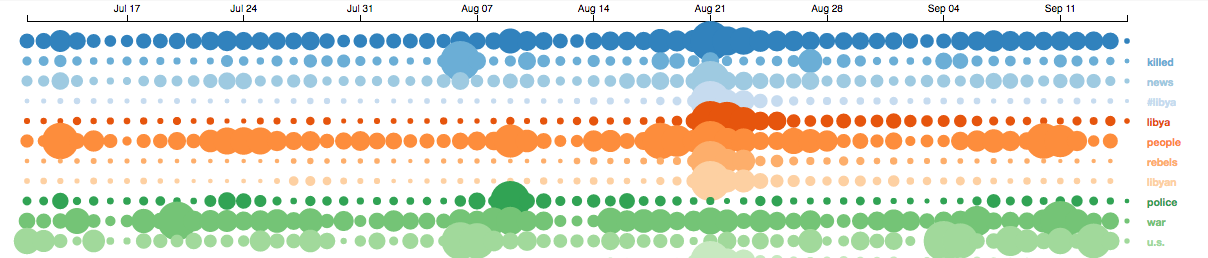
\includegraphics[width=1.0\textwidth]{img/screenShot.png}
    \caption{An illustration of the time series of Military related states on Twitter dataset from 2011-06-30 to 2011-09-15.}
\end{figure*}
\end{comment}

\subsection{Quantitive Study}
\textbf{Data set.} We conduct the empirical analysis on a twitter dataset which is constructed by \cite{petrovic2012using} and widely used by previous event detection researches \cite{petrovic2013can} \cite{Wurzer:2015wq}. 
Due to the developer policy of Twitter\footnote{https://dev.twitter.com/overview/terms/policy}, \cite{petrovic2012using} only redistributes tweets' IDs\footnote{http://demeter.inf.ed.ac.uk/cross/docs/fsd\_corpus.tar.gz}.
We collected the tweets' contents according to the IDs with the help of Twitter API. 

%TODO
The benchmark \textit{Edinburgh twitter corpus} contains 27 manually labeled events\cite{petrovic2013can}\footnote{\url{http://demeter.inf.ed.ac.uk/cross/docs/Newswire_Events.tar.gz}} and 90 million tweets. Though we cannot get the whole dataset due to the limit of Twitter API, after neccessary pre-processing, our rebuilt dataset still contains 36,627,434 tweets, which spans identically from 2011/06/30 to 2011/09/15, and also covers 27 labeled events.
More details of the original dataset are described in \cite{petrovic2010edinburgh}.
\begin{comment}
20-newsgroup\footnote{http://qwone.com/~jason/20Newsgroups/}

NPMI\cite{Aletras2013EvaluatingTC}\cite{Rder2015ExploringTS}\footnote{https://github.com/AKSW/Palmetto}.

\textbf{Benchmark1} The first set of the ground truth about events in the corpus are provided by \cite{petrovic2013can}, which is mentioned above. 
And 27 events ...

\textbf{Benchmark2} here.

\textbf{Normal States Initialization} here.

\textbf{Baseline}

UMass System\cite{Allan:2000wu}

LSH

TimeUserLDA

Twevent

EDCoW

BBTM\cite{yan2015probabilistic}

\textbf{Model Setting}
\end{comment}
%\textbf{Topic Coherence} \cite{roder2015exploring}
\subsection{Qualitative Study}
%\textbf{PMI}
%\subsection{Evaluation of Detected Events}
\begin{comment}
\textbf{Precision} Precision@Benchmark1, Precision@Benchmark2

\textbf{Recall}

\textbf{Accuracy}

\textbf{DERate(Duplicate Event Rate)}
\end{comment}
%\subsection{Case Study}


%\subsection{Application on Reddit}

\section{Conclusions \& Future Work}



\bibliographystyle{named}
\small
\bibliography{paperbib}


\end{document}
